\section{Модель Кейна--Меле}
	Модель Кейна--Меле --- это плоская шестиугольная решётка со спин--орбитальным
	взаимодействием. 
	Её гамильтониан --- 
	\begin{equation}
		\hat{H} = 
			\sum_{\langle ij \rangle \alpha} t c^\dagger_{i\alpha} c_{j\alpha} + 
				\sum_{\langle\langle ij \rangle\rangle \alpha\beta} 
					it_2 \nu_{ij} s^z_{\alpha \beta} c^\dagger_{i\alpha} c_{i\beta}
	\end{equation}
	Суммирование в первом слагаемом идёт по соседним ячейкам, а во втором --- по соседним
	ячейкам \emph{одной подрешётки}, при этом $\nu_{ij} = \pm 1$, и его знак зависит
	от ориентации кратчайшего пути, соединяющего две ячейки. Это наиболее просто показать
	на рисунке.

	Модель Кейна--Меле удовлетворяет всем 
	свойствам симметрии из предыдущего раздела. Более
	того, все модели шестиугольной решётки с этими симметриями будут отличаться от модели
	Кейна--Меле только наличием более ``далёких'' матричных элементов.

	Части гамильтониана, отвечающие разным спинам, как уже было отмечено в предыдущем
	разделе, независимы.
	Запишем гамильтониан для $s = +1$ в менее компактном, но более удобном виде:
	\begin{multline}
		H = t\sum a_{mn}^\dagger(b_{mn} + b_{m,n-1} + b_{m+1,n-1}) + \mbox{h.c.} \\
		+it_2 \sum a_{mn}^\dagger(a_{m,n+1} + a_{m-1,n} + a_{m+1,n-1}) + \mbox{h.c.} \\
		-it_2 \sum b_{mn}^\dagger(b_{m,n+1} + b_{m-1,n} + b_{m+1,n-1}) + \mbox{h.c.} 
	\end{multline}
	Операторы $a$, $b$ ``сидят`` в узлах шестиугольной решётки, базис которой выбран так:
	\begin{equation}
		\vec{x} = \left(\begin{matrix} \frac32 \\ \frac{\sqrt{3}}{2} \end{matrix}\right), \quad
		\vec{y} = \left(\begin{matrix} 0 \\ \sqrt{3} \end{matrix}\right)
	\end{equation}

	\begin{wrapfigure}{r}{0.5\textwidth}
		\begin{center}
		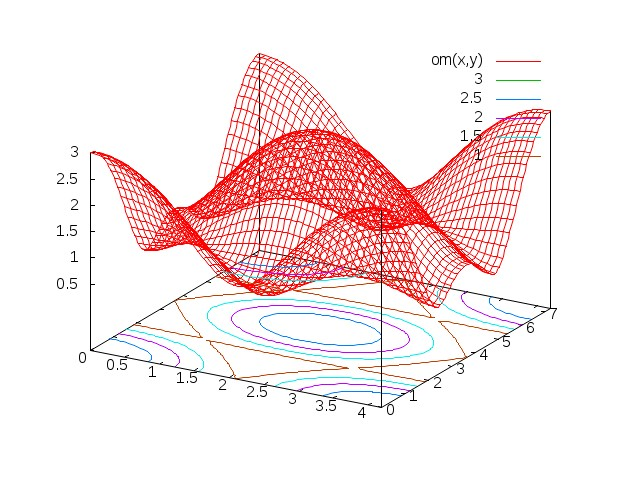
\includegraphics[width=0.46\textwidth]{haldane_spectrum.jpg}
		\end{center}
	\end{wrapfigure}

	После преобразования Фурье гамильтониан будет задаваться матрицей
	\begin{equation}
		\left(
		\begin{matrix}
			\xi && \eta e^{i\phi} \\
			\eta e^{-i\phi} && -\xi
		\end{matrix}
		\right),
	\end{equation}
	\begin{equation}
		\xi = 2t_2 (\sin{px} - \sin{py} - \sin{p(x-y)}) 
	\end{equation}
	\begin{equation}
		\eta e^{i\phi} = t(1 + e^{-ipy} + e^{ip(x-y)}) 
	\end{equation}
	Энергия, таким образом,
	\begin{multline}
		\epsilon_p^2 = \xi^2 + \eta^2 =\\
			= 4t_2^2(\sin{px} - \sin{py} - \sin{p(x-y)})^2 + 
					t^2 |1 + e^{-ipy} + e^{ip(x-y)}|^2
		\label{spectrum}
	\end{multline}
	
	Спектр, определяемый формулой (\ref{spectrum}), изображён на рисунке. 

	\subsection{Краевые состояния}
	Чтобы исследовать полосу из атомов в этой модели, удобно сделать преобразование Фурье
	только по одной координате:
	\begin{equation}
		a_{mn} = \sum \frac{e^{i\sqrt{3}p_yn}}{\sqrt{N}} a_{m,p_y}
	\end{equation}
	(и то же самое для $b$). Тогда гамильтониан запишется так:
	\begin{multline}
		H = \sum_{m, p_y} t(1+e^{-i\sqrt{3}p_ya}) a_m^\dagger b_m
		 + te^{-i\sqrt{3}p_ya} a_m^\dagger b_{m+1} + \mbox{h.c.} \\
		- 2t_2 \sin{\sqrt{3} p_ya} (a_m^\dagger a_m -  b_m^\dagger b_m)\\
		+ it_2(1 - e^{i\sqrt{3}p_ya}) (a_m^\dagger a_{m-1} - b_m^\dagger b_{m-1}) 
		+ \mbox{h.c}
	\end{multline}

	\begin{figure}[h]
		\begin{center}	
			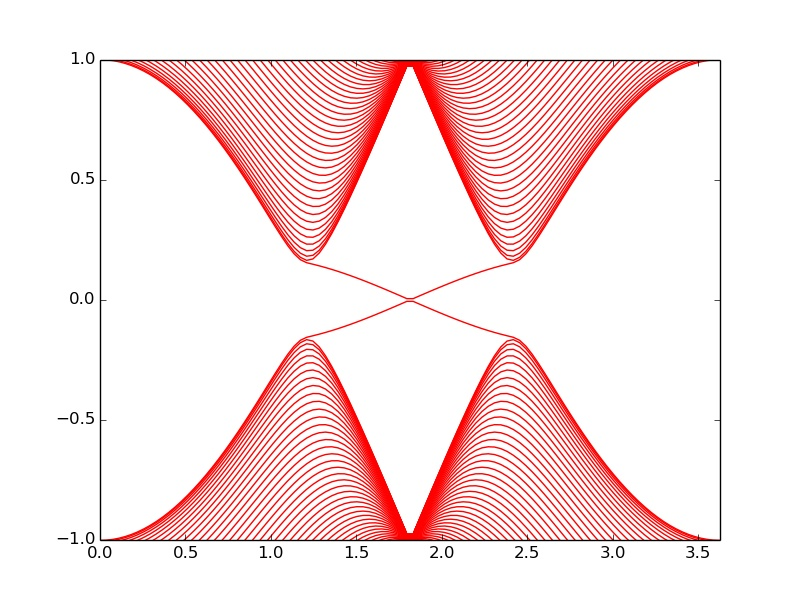
\includegraphics[width=0.5\textwidth]{levels.jpg}
		\end{center}
	\end{figure}

	Для цепочки длиной в несколько десятков атомов собственные значения легко найти на 
	компьютере. Для $t = 1$, $t_2 = 0.03$ уровни 
	энергии изображены на рисунке.
	В статье \cite{Kane2005} приведена картинка для точно таких же данных. Она полностью
	совпадает с приведённой здесь.
	
	Тот же вид дисперсионного соотношения можно получить и аналитически. Это делается по 
	точно тому же алгоритму, что и раньше, правда, формулы получаются значительно более
	громоздкие.

	Формулу для энергии можно переписать в виде
	\begin{multline}
		\epsilon_p^2 = \left(4t_2\sin{\frac{\sqrt{3}p_ya}{2}} \cos{\frac{3p_xa}{2}} - 
				4t_2\sin{\frac{\sqrt{3}p_ya}{2}} \cos{\frac{\sqrt{3}p_ya}{2}} +
				\frac{t^2}{2t_2} \cot{\frac{\sqrt{3}p_ya}{2}}\right)^2\\
				- \frac{t^4}{4t_2^2}\cot^2{\frac{\sqrt{3}p_ya}{2}}
				+ t^2\left(1 + 8\cos^2{\frac{\sqrt{3}p_ya}{2}}\right) = \\
				= \left(a\cos{\frac{3p_xa}{2}} + b\right)^2 + c
	\end{multline}
	Это значит, что функции Грина в импульсном представлении ---
	\begin{equation}
		\begin{split}
		G^R_0(\omega,A,A, \vec{p}) = \frac{\omega + \xi}{\omega^2 - \epsilon_p^2 + i\delta}\\
		G^R_0(\omega,B,B, \vec{p}) = \frac{\omega - \xi}{\omega^2 - \epsilon_p^2 + i\delta}\\
		G^R_0(\omega,A,B, \vec{p}) = 
			\frac{\eta e^{-i\phi}}{\omega^2 - \epsilon_p^2 + i\delta}\\
		G^R_0(\omega,B,A, \vec{p}) = G^R_0(\omega,A,B, -\vec{p})^{*}\\
		\end{split}
	\end{equation}
	Теперь перейдём к рассмотрению границы цепочки. 
	Пусть граница идёт вдоль вектора $\vec{y}$.
	Тогда уравнение Дайсона распадётся на независиме уравнения 
	на функции $G(m,m',p_y)$. Границу
	можно реализовать, введя бесконечные добавки к энергии для атомов обоих типов вдоль
	одной линии.
	\begin{multline}
		G^R(m,s,m',s',p_y) = G^R_0(m,s,m',s'p_y)  \\
			+\Delta E G^R_0(m,s,0,A,p_y)G^R(0,A,m',s',p_y)  \\
						+\Delta E G^R_0(m,s,0,B,p_y)G^R(0,B,m',s',p_y) 
	\end{multline}
	Для бесконечного $\Delta E$ уравнение на связанные состояния ---
	\begin{equation}
		\label{det}
		\operatorname{det} 
		\left(\begin{matrix}
			G^R_0(0,A,0,A,p_y) & G^R_0(0,A,0,B,p_y) \\
			G^R_0(0,B,0,A,p_y) & G^R_0(0,B,0,B,p_y) 
		\end{matrix}\right) = 0
	\end{equation}
	Таким образом, остаётся вычислить функции Грина, входящие в детеримнант. Вычисляются они 
	по таким формулам:
	\begin{equation}
		G_0^R(m,s,m',s',p_y) = 
			\nu_x\int \frac{dp_x}{2\pi} e^{i\vec{p}\vec{x}(m-m')} G^0_R(s,s',p_x,p_y)
	\end{equation}
	Этот интеграл равен сумме по полюсам в верхней полуплоскости, 
	которые определяются уравнением
	\begin{equation}
		\omega^2 = (a\cos{k} + b)^2 + c
	\end{equation}

	\begin{figure}[h]
		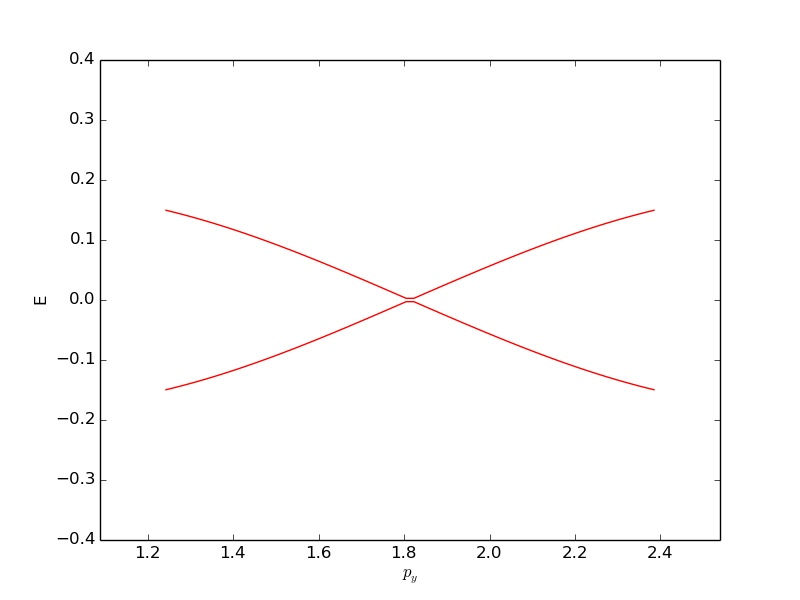
\includegraphics[width=0.40\textwidth]{edge_kanemele.jpg}
	\end{figure}
	Окончательные формулы весьма громоздки, поэтому приводить здесь мы их не будем. Уравнение
	\eqref{det} после всех подстановок становится обыкновенным алгебраическим уравнением.
	Оно решается на компьютере, и в результате снова получается знакомая нам зависимость 
	энергии от квазиимпульса.

	\subsection{Отсутствие рассеяния для краевых состояний}
	После рассмотрения технических деталей того, как получить дисперсионное соотношение,
	обратимся к его физическому смыслу. На обоих рисунках присутствует две ветви,
	соответствующие краевым состояниям. В обоих случаях состояния, соответствующие этим
	ветвям, пространственно разнесены: в случае полосы состояния находятся на её разных
	краях, а в случае разделённой полуплоскости и вовсе находятся на её разных половинах.
	Таким образом, краю реально соответствует \emph{одна} ветвь спектра, соответствующая
	распространению в выделенном направлении.

	Здесь нужно вспомнить о том, что рассматривалась только одна ''половина`` гамильтониана,
	соответствующая $s = 1$. Спину $s = -1$ соответствует комплексно сопряжённый
	гамильтониан, что означает, что соответсвующее краевое состояние будет распространяться
	в противоположном направлении.
	
	Таким образом, окончательная картина такова: направление движения электрона по границе
	решётки находится в однозначном соответствии с его спином. К тому же, состояния,
	отличающиеся направлением движения (и спина), переходят друг в друга при обращении
	времени.

	Замечательный факт состоит в том, что из--за симметрии относительно обращения времени
	никакое возмущение не может заставить эти состояния рассеяться друг в друга (см.
	\cite{Kane2005})

	Однако необходимым условием при построении модели Кейна--Меле было то, что в качестве
	атомных орбиталей выбираются s-орбитали. Дело в том, что только s--орбитали являются 
	собственными состояниями для проекции спина (см. \cite{LL_KED}). 
	Поэтому представляет интерес построение
	модели с явным учётом p-зон.
